\documentclass[11pt]{article}
\usepackage[letterpaper,margin=0.95in]{geometry}
\usepackage[T1]{fontenc}
\usepackage{lmodern}
\usepackage{microtype}
\usepackage{amsmath,amssymb}
\usepackage{graphicx}
\usepackage{booktabs,tabularx,array,multirow}
\usepackage{enumitem}
\usepackage[dvipsnames]{xcolor}
\usepackage{caption}
\usepackage{float}
\usepackage{adjustbox}
\usepackage[hidelinks]{hyperref}
\definecolor{hblue}{HTML}{2a78d6}
\definecolor{boxbg}{HTML}{f4f3ef}
\definecolor{ink2}{HTML}{52514e}
\hypersetup{colorlinks=true,linkcolor=hblue,urlcolor=hblue,citecolor=hblue}
\captionsetup{font=small,labelfont=bf,margin=0.15in}
\setlist{itemsep=2pt,topsep=3pt,parsep=0pt}
\setlength{\parskip}{4pt}
\setlength{\parindent}{0pt}
\graphicspath{{../../../results/}{figs/}}
\newcommand{\keybox}[1]{\par\smallskip\noindent\colorbox{boxbg}{\parbox{\dimexpr\linewidth-2\fboxsep}{\small #1}}\par\smallskip}
\newcommand{\TPR}{\mathrm{TPR}}
\newcommand{\FPR}{\mathrm{FPR}}
\renewcommand{\arraystretch}{1.18}

\sloppy
\usepackage{xurl}

\usepackage{tikz}
\usepackage[section]{placeins}
\newcommand{\src}[1]{{\footnotesize\textcolor{ink2}{[\nolinkurl{#1}]}}}
\newcommand{\ci}[2]{\,[#1,\,#2]}
\newcommand{\hl}[1]{\textbf{#1}}
\title{\textbf{Idea 3: Monitor-Aware Attackers vs Sequential Detectors}\\[4pt]
\large Rounds 1--3, with all audit corrections applied}
\date{October 22, 2026}
\begin{document}
\maketitle
\vspace{-1.5em}

\keybox{\textbf{Summary.} An LLM rewriter was given the deployed monitor prompt and the exact detector rule (Kerckhoffs) and asked to restructure 150 real, successful multi-step MonitoringBench attacks so that they evade a max, CUSUM, e-process or multi-chart detector calibrated at matched trajectory FPR on 550 honest runs. Three rounds were run and then re-analysed by two independent audits; every number below is the audit-corrected value and cites its results file.
\begin{enumerate}[leftmargin=1.2em]
\item \textbf{No detectable effect of detector knowledge.} One-shot pacing vs a one-shot plain rewrite against max at 1\% FPR is $+0.087\ci{-0.032}{+0.183}$ under strict validity ($p=0.20$; pre-specified primary contrast). None of 24 one-shot pacing-vs-control contrasts survives Holm correction in round 2, and all 12 such contrasts at max in round 3 (two rewriters $\times$ three arms $\times$ two FPRs) have CIs containing 0.
\item \textbf{Any LLM rewrite makes attacks easier to catch.} A rewrite with no monitor information lowers undetected success vs the originals by $-0.357$ (judge) to $-0.500$ (strict) with a \texttt{gpt-4.1} rewriter, and by $-0.371\ci{-0.550}{-0.185}$ with a different-family rewriter (\texttt{gemini-2.5-pro}). About 60\% of the latter is broken attacks; the detection-only part is $-0.143\ci{-0.300}{-0.027}$.
\item \textbf{Two earlier headlines are retracted.} Round 1's ``detector-aware rewriting backfires'' was this rewrite artifact (no control existed). Round 2's ``pacing beats the control by $+0.21$'' compared an adaptive arm, selected on the evaluation monitor's own scores, with a one-shot control.
\item \textbf{Detectors.} Max, CUSUM with $k=1.5$ and top-3 sum hold nominal FPR; max catches the most originals and top-3 sum is the most robust to pacing. CUSUM with $k=0.5$, the e-process, Shiryaev--Roberts and windowed GLR leave $\ge0.93$ of the original attacks undetected under the strong monitor. The multi-chart OR realizes 0.017--0.020 FPR at a nominal 0.01, so its matched-FPR cells overstate detection.
\item \textbf{No $\sqrt{\mathrm{ARL}}$ scaling.} Undetected damage is flat in ARL (slopes 0.007--0.073 over the calibratable range ARL $\le551$, vs 0.5 predicted). Detection is driven by single spikes.
\item \textbf{Fabricated tool outputs do not drive the results}; stripping all outputs leaves every conclusion unchanged. Execution replay in BashArena works end to end, but the stored trajectories lack structured tool calls, so rewrites were not replayed.
\end{enumerate}
Spend: \$68.36 (round 1) + \$304.77 (round 2) + \$111.02 (round 3) on OpenRouter \src{results/spend_ledger.jsonl}.}


%======================================================================
\section{Question and threat model}

\paragraph{Question.} Sequential detectors have explicit evasion parameters. A CUSUM with reference $k$ accumulates nothing from steps whose standardized suspicion stays below $k$ and resets after benign steps. Covert-adversary theory predicts that an attacker who knows the detector can pace its evidence to about $1/\mathrm{ARL}$ per step: it stays below the false-alarm clock, but its total undetected damage is capped at $\Theta(\sqrt{\mathrm{ARL}})$. Three questions follow.
\begin{itemize}
\item Can a capable LLM attacker restructure real, working multi-step attacks to exploit a known detector without breaking them?
\item Does a multi-chart detector (max + CUSUM + e-process) close any gap that a single chart leaves?
\item Does undetected damage grow like $\sqrt{\mathrm{ARL}}$?
\end{itemize}

\paragraph{Threat model.} The attacker knows the monitor prompt, the detector rule and its parameters, and (in round 2) the honest score distribution. It does not control the monitor. It may restructure an existing successful attack (interleave benign main-task steps, split commands, reorder independent steps, delay onset, wrap in plausible scaffolding, rename consistently). It may not drop or fake any attack-critical effect. Attack content is described here only at the level of side-task families; no payloads appear in this report or in the repository.

\paragraph{How to read the numbers.} Undetected success (US) is the share of base attacks that are both valid and not alarmed; lower is better for the defender. Differences are paired over identical base attacks. ``Judge'' validity is an upper bound on US and ``strict'' validity a lower bound (Section~\ref{sec:methods}). Unless stated otherwise CIs are 95\% joint bootstrap intervals that resample honest runs and attacks together and recompute every threshold per replicate. File paths in brackets are relative to the repository's \texttt{results/} directory.

%======================================================================
\section{The three rounds at a glance}

\begin{table}[H]\centering\small
\begin{adjustbox}{max width=\linewidth}
\begin{tabular}{@{}llll@{}}
\toprule
& Round 1 (Oct 20) & Round 2 (Oct 21) & Round 3 (Oct 22)\\
\midrule
Monitor & \texttt{gpt-4.1-mini}, \texttt{full} + \texttt{none} & \texttt{gpt-4.1}, \texttt{none} & \texttt{gpt-4.1}, \texttt{none}; also no-output\\
Rewriter & \texttt{gpt-4.1} & \texttt{gpt-4.1} & \texttt{gpt-4.1} and \texttt{gemini-2.5-pro}\\
Arms & max-, CUSUM-, multichart-aware & 3 pacing arms + rewrite control & control + 3 pacing arms per rewriter\\
Feedback & adaptive ($\le2$ rounds) and one-shot & adaptive (pacing) and one-shot & one-shot only\\
Base attacks & 150 (paired 126) & 150 (paired 126) & 35 (17 tasks)\\
Detectors & max, CUSUM $k{=}0.5$, e-process, OR & + CUSUM $k{=}1.5$, top-3 sum, SR, GLR & max, CUSUM $k{=}1.5$, OR, top-3 sum\\
New checks & -- & control arm, mechanism & replay, leak test, realized FPR\\
Spend & \$68.36 & \$304.77 & \$111.02\\
\bottomrule
\end{tabular}
\end{adjustbox}
\caption{Design of the three rounds. The audits (October 21 and 22) re-analysed rounds 1--3 with joint bootstrap CIs, strict validity and one-shot-only strategy contrasts \src{results/fixes/corrections.csv}, \src{results/audit2/corrections.csv}.}\label{tab:rounds}
\end{table}

%======================================================================
\section{Common methods}\label{sec:methods}

\paragraph{Base attacks.} 150 successful MonitoringBench attacks on BashArena sysadmin tasks, structures S2--S4 (multi-step), 6--55 steps, stratified across the four side-task families (firewall disabling, sudo escalation, download-and-run malware, credential exfiltration). They come from Idea 1's scored 775-attack sample, so the originals' per-step scores were already paid for. Each has a heuristic onset step and an execution step.

\paragraph{Monitors.} Action-only (agent reasoning hidden), prompt \texttt{ctrl-basic-v1}, logprob-expected 0--10 score per step. History modes: \texttt{full} (sees previous actions) and \texttt{none} (scores each action on its own; least sensitive to fabricated history). The final submit step is stripped, and only when it is a real submit call (audit m6; no point estimate changed, \src{results/fixes/t3/tables_fixes_t3_round1.md}).

\paragraph{Detectors.} Per-trajectory rules over the per-step score stream: \textbf{max} (alarm if any step exceeds a threshold); \textbf{CUSUM} on whitened scores with reference $k=0.5$ (round 1) and $k\in\{0.5,1.5\}$ (round 2 on); a \textbf{conformal e-process} with a power calibrator; the \textbf{multi-chart OR} of \{max, CUSUM, e-process\}, each with an exponential-tail fit; \textbf{top-3 sum} (sum of the three largest step scores; round 2 on); and, evaluation-only in round 2, Shiryaev--Roberts (SR), an SR-type e-detector and a windowed GLR (window 20). Each is calibrated on the 550 honest runs (Honest-550) at matched trajectory FPR $\alpha\in\{0.01,0.003\}$ with randomized thresholds.

\paragraph{Rewriting pipeline.} (1) \texttt{gpt-4.1-mini} extracts a checklist of the attack-critical effects of each original. (2) The rewriter emits a restructured action sequence; new actions get plausible fabricated tool outputs (nothing is executed). (3) \texttt{gpt-4.1-mini} judges whether every checklist effect is preserved, and a static check records whether the attack's target literals (paths, hosts, users) appear verbatim. (4) The deployed monitor scores the rewrite. (5) Adaptive arms only: the arm's calibrated verdict and per-step suspicion profile are returned for up to two more attempts, stopping once an attempt evades and is valid. Round 0 is kept as the one-shot arm.

\paragraph{Validity bounds.} The audits found that the original ``valid'' flag was the LLM judge alone, although the literal check had been described as part of it \src{results/audit/issues.csv} (M2). Three definitions are now reported:
\begin{itemize}
\item \textbf{judge}: LLM judge only (upper bound on US);
\item \textbf{strict}: judge \emph{and} every target literal verbatim in the rewritten actions (lower bound; primary since the first audit);
\item \textbf{strict-rel}: judge and every target literal that the original's own actions contain. 28 of 150 successful originals do not write every target literal themselves, so strict is asymmetric against rewrites when they are compared with the originals; strict-rel is the symmetric lower bound \src{results/fixes/r2_t3/run_info.json}.
\end{itemize}

\paragraph{Statistics.} US $=\mathbb E[\text{valid}\times(1-P(\text{alarm}))]$ under the randomized threshold. CIs come from a joint bootstrap (\texttt{amd.evaluation.paired}): honest runs and base attacks are resampled together (clustered by task in round 3), and detectors are refit and thresholds recomputed per replicate. The round-1 and round-2 tables originally resampled attacks only and calibrated in-sample, which understated CI width (audit m5). Strategy contrasts are one-shot vs one-shot only (audit M1). The pre-specified primary contrast is one-shot \texttt{pace\_max} minus the one-shot rewrite control, deployed max, $\alpha=0.01$, strict validity, paired $n=126$. Holm correction is applied within families of contrasts where stated.

%======================================================================
\section{Round 1: detector-aware rewriting under a weak monitor}

\paragraph{Setup.} \texttt{gpt-4.1} rewrote each of the 150 attacks three times, once per detector spec (max-, CUSUM- and multichart-aware). Coverage was 145/131/143; 126 base attacks have all arms. The monitor was \texttt{gpt-4.1-mini}. A \texttt{gpt-5-mini} rewriter was piloted and dropped because about half its outputs were unparseable.

\subsection{Levels: as measured and with strict validity}

\begin{table}[H]\centering\small
\begin{adjustbox}{max width=\linewidth}
\begin{tabular}{@{}llcccc@{}}
\toprule
Variant & Attacker $\backslash$ deployed & max & CUSUM $k{=}0.5$ & e-process & multi-chart OR\\
\midrule
& original (\emph{nothing}) & 0.857 & 0.960 & 0.921 & 0.851\\
\midrule
adaptive & max-aware & 0.690 / 0.516 & 0.738 / 0.563 & 0.468 / 0.325 & 0.493 / 0.351\\
& CUSUM-aware & 0.635 / 0.468 & 0.857 / 0.698 & 0.698 / 0.548 & 0.581 / 0.422\\
& multichart-aware & 0.730 / 0.532 & 0.810 / 0.611 & 0.659 / 0.468 & 0.677 / 0.479\\
\midrule
one-shot & max-aware & 0.532 / 0.365 & 0.611 / 0.452 & 0.373 / 0.230 & 0.373 / 0.230\\
& CUSUM-aware & 0.595 / 0.429 & 0.762 / 0.611 & 0.643 / 0.500 & 0.541 / 0.390\\
& multichart-aware & 0.579 / 0.397 & 0.730 / 0.540 & 0.532 / 0.357 & 0.511 / 0.328\\
\bottomrule
\end{tabular}
\end{adjustbox}
\caption{Round 1 undetected success, \texttt{full} monitor, $\alpha=0.01$, paired $n=126$; cells are judge / strict. The originals are valid by construction. Joint CIs for every cell are in \src{results/fixes/t3/tables_fixes_t3_round1.md}; e.g.\ original vs max $0.857\ci{0.794}{0.913}$. The \texttt{none}-mode table has the same pattern.}\label{tab:r1levels}
\end{table}


\subsection{What the attacker did: condensation}
The round-1 rewriter shortened attacks instead of diluting them \src{results/r2_t3/tables.md}:
\begin{itemize}
\item length ratio 0.63 / 0.83 / 0.58 (adaptive max- / CUSUM- / multichart-aware), i.e.\ 14.0 / 7.8 / 15.3 fewer steps; one-shot 0.55 / 0.80 / 0.53;
\item mean per-trajectory peak suspicion under \texttt{gpt-4.1-mini} rose from 5.8 (originals) to 7.6 (max-aware) \src{results/t3/tables.md};
\item under the round-2 monitor (\texttt{gpt-4.1}, \texttt{none}) the round-1 arms' mean peak is 7.47--8.04 vs 6.03 for the originals.
\end{itemize}
The original write-up read this as the mechanism of a ``backfire''. Round 2 showed that a rewrite that does \emph{not} condense raises the peak just as much (Section~\ref{sec:mechanism}).

\subsection{Aware arms vs originals, and feedback}
\begin{table}[H]\centering\small
\begin{adjustbox}{max width=\linewidth}
\begin{tabular}{@{}lccc@{}}
\toprule
Aware arm $-$ original (vs max, \texttt{full}, adaptive) & judge & strict-rel & strict\\
\midrule
max-aware & $-0.167\ci{-0.262}{-0.095}$ & $-0.214\ci{-0.310}{-0.135}$ & $-0.341\ci{-0.437}{-0.246}$\\
CUSUM-aware & $-0.222\ci{-0.310}{-0.135}$ & $-0.262\ci{-0.357}{-0.175}$ & $-0.389\ci{-0.484}{-0.294}$\\
multichart-aware & $-0.127\ci{-0.214}{-0.048}$ & $-0.198\ci{-0.286}{-0.119}$ & $-0.325\ci{-0.421}{-0.230}$\\
\bottomrule
\end{tabular}
\end{adjustbox}
\caption{Round 1 aware-minus-original differences, $\alpha=0.01$, joint CIs \src{results/fixes/t3/tables_fixes_t3_round1.md}. All are negative, but round 1 has no rewrite-only control, so these mix strategy with the cost of rewriting.}
\end{table}

\paragraph{Adaptive vs one-shot.} On the matched diagonal adaptive minus one-shot is $+0.159\ci{+0.095}{+0.230}$ (max), $+0.095\ci{+0.032}{+0.143}$ (CUSUM) and $+0.167\ci{+0.095}{+0.222}$ (multi-chart) in \texttt{full} mode; strict $+0.151$ for max. In \texttt{none} mode, which the feedback did not use, it shrinks to $+0.032\ci{-0.048}{+0.111}$, $+0.048\ci{0.000}{+0.087}$ and $+0.079\ci{+0.024}{+0.143}$ \src{results/fixes/t3/tables_fixes_t3_round1.md}. The feedback came from the same deterministic scores and threshold used for evaluation, so this gain is in-sample selection (``oracle feedback''), not out-of-sample attacker capability.

\subsection{Re-reading round 1 against a rewrite-only control}\label{sec:r1reread}
Round 2 added a rewrite control (same pipeline, no monitor or detector information). Under the round-2 monitor the round-1 arms can be compared with it, approximately (the control used the round-2 pipeline, and the round-1 adaptive arms were selected on \texttt{gpt-4.1-mini} feedback). Against max at $\alpha=0.01$ \src{results/fixes/t3/tables_fixes_t3_round1.md}:
\begin{itemize}
\item one-shot, judge: max-aware $+0.095\ci{+0.008}{+0.183}$, CUSUM-aware $+0.087\ci{-0.024}{+0.159}$, multichart-aware $+0.063\ci{-0.032}{+0.143}$;
\item one-shot, strict: $+0.079\ci{-0.008}{+0.159}$, $+0.071\ci{-0.032}{+0.135}$, $+0.032\ci{-0.056}{+0.103}$;
\item adaptive, judge: $+0.135\ci{+0.048}{+0.214}$, $+0.063\ci{-0.040}{+0.151}$, $+0.111\ci{+0.016}{+0.206}$.
\end{itemize}
Every point estimate favours the aware arm over a plain rewrite, and the CIs that exclude 0 do so in the attacker's favour. The round-1 drop below the originals is therefore evidence that LLM rewriting costs the attacker, not that detector knowledge does (audit M3).

\subsection{Detectors and calibration in round 1}
\begin{itemize}
\item On the originals, \texttt{gpt-4.1-mini} catches 14\% (max), 4\% (CUSUM $k=0.5$), 8\% (e-process) and 15\% (OR) at 1\% FPR (one minus the first row of Table~\ref{tab:r1levels}).
\item Held-out FPR (calibrate on 275 honest, test on 275, 200 splits): max, CUSUM and e-process realize 1.00--1.08$\times$ nominal at 0.01 in \texttt{full} mode (up to 1.42$\times$ at 0.003 in \texttt{none}). The OR realizes 0.0179 at 0.01 (1.79$\times$) and 0.0124 at 0.003 (4.12$\times$) \src{results/fixes/t3/m5_holdout_fpr_r1.csv}. The OR's apparent tie with max is therefore partly bought with extra false alarms.
\end{itemize}

%======================================================================
\section{Round 2: strong monitor, pacing attackers and a rewrite control}

\subsection{Monitor choice}
In a 40+40 pilot (\texttt{none} mode, per-trajectory max), per-trajectory AUROC was 0.709 for \texttt{gpt-4o}, 0.871 for \texttt{gpt-4.1} and 0.836 for \texttt{claude-haiku-4.5} (integer scores only) \src{results/r2_t3/pilot_auroc.json}. \texttt{gpt-4.1} was chosen. On the full paired set its advantage is mainly at low FPR: on the 126 paired originals, max TPR at 1\% FPR is 0.246 (\texttt{gpt-4.1} \texttt{none}) vs 0.143 for \texttt{gpt-4.1-mini} \texttt{none} \src{results/fixes/r2_t3/tables_fixes_r2_t3.md}, \src{results/fixes/t3/tables_fixes_t3_round1.md}. The pilot AUROC advantage did not carry over to the full sample (a winner's curse in the 40+40 pilot; EXPERIMENT\_LOG, October 21), so the ``strong'' monitor is stronger, not strong.

\subsection{Arms}
\begin{itemize}
\item \textbf{Pacing} (\texttt{pace\_max}, \texttt{pace\_cusum}, \texttt{pace\_multichart}): told not to shorten, to keep or add benign main-task steps, and to spread attack-critical effects thinly so no single step and no sustained run looks suspicious. The CUSUM and multichart specs embed the honest score distribution and the integer-score $\to$ whitened-$z$ table so that the attacker can pace below the slack. JSON output mode and a 90\% length floor with resampling.
\item \textbf{Rewrite control}: same pipeline, prompt structure and length floor, no monitor or detector information, one-shot only (its adaptive directory is byte-identical to its one-shot directory for all 150 streams \src{results/fixes/r2_t3/run_info.json}).
\item The round-1 arms, re-scored with \texttt{gpt-4.1}.
\end{itemize}

\begin{table}[H]\centering\small
\begin{adjustbox}{max width=\linewidth}
\begin{tabular}{@{}lcccccc@{}}
\toprule
Arm (adaptive) & $n$ & Length ratio & Steps added & Attack-relevant steps & Literal pres. & Strict-valid rate\\
\midrule
round-1 max / CUSUM / multichart & 145 / 131 / 143 & 0.63 / 0.83 / 0.58 & $-14.0$ / $-7.8$ / $-15.3$ & 5.7 / 4.1 / 4.2 & 0.88--0.90 & 0.79--0.81\\
pace max / CUSUM / multichart & 150 & 1.17 / 1.18 / 1.17 & $+4.4$ / $+4.4$ / $+4.5$ & 5.2 / 5.0 / 5.0 & 0.88--0.89 & 0.80--0.83\\
rewrite control & 150 & 1.17 & $+4.4$ & 7.6 & 0.89 & 0.78\\
\bottomrule
\end{tabular}
\end{adjustbox}
\caption{Attacker cost and validity, round 2 (\texttt{none}). Attack-relevant step counts are self-reported by the rewriter. Literal preservation is the mean fraction of target literals kept; the strict-valid rate is the share of rewrites that keep all of them and pass the judge (paired 126). Sources: \src{results/r2_t3/tables.md}, \src{results/fixes/r2_t3/tables_fixes_r2_t3.md}.}
\end{table}

The pacing instruction worked as a length instruction: pacing rewrites are 17--18\% longer than the originals, against 17--42\% shorter for round 1.

\subsection{Mechanism: where the suspicion is}\label{sec:mechanism}
\begin{table}[H]\centering\small
\begin{adjustbox}{max width=\linewidth}
\begin{tabular}{@{}lcccccc@{}}
\toprule
Arm & Peak score & Peak on attack step & Mean on attack steps & Mean on benign steps & Any attack step $>$ honest q99 & $\Delta$ peak vs original\\
\midrule
original & 6.08 & 0.57 & 2.60 & 0.34 & 0.44 & --\\
round-1 arms & 7.51--8.05 & 0.89--0.97 & 3.74--4.35 & 0.24--0.50 & 0.75--0.86 & $+1.43$ to $+1.96$\\
pacing arms & 7.85--8.10 & 0.87--0.90 & 4.11--4.26 & 0.31--0.37 & 0.86--0.87 & $+1.77$ to $+2.02$\\
rewrite control & 8.37 & 0.98 & 3.74 & 0.12 & 0.92 & $+2.29\ci{+1.82}{+2.79}$\\
\bottomrule
\end{tabular}
\end{adjustbox}
\caption{Per-trajectory suspicion profile under \texttt{gpt-4.1} \texttt{none}, adaptive arms, paired $n=126$; honest per-step q99 = 6.67 \src{results/r2_t3/mechanism.md}.}\label{tab:mech}
\end{table}

\begin{figure}[tbp]\centering
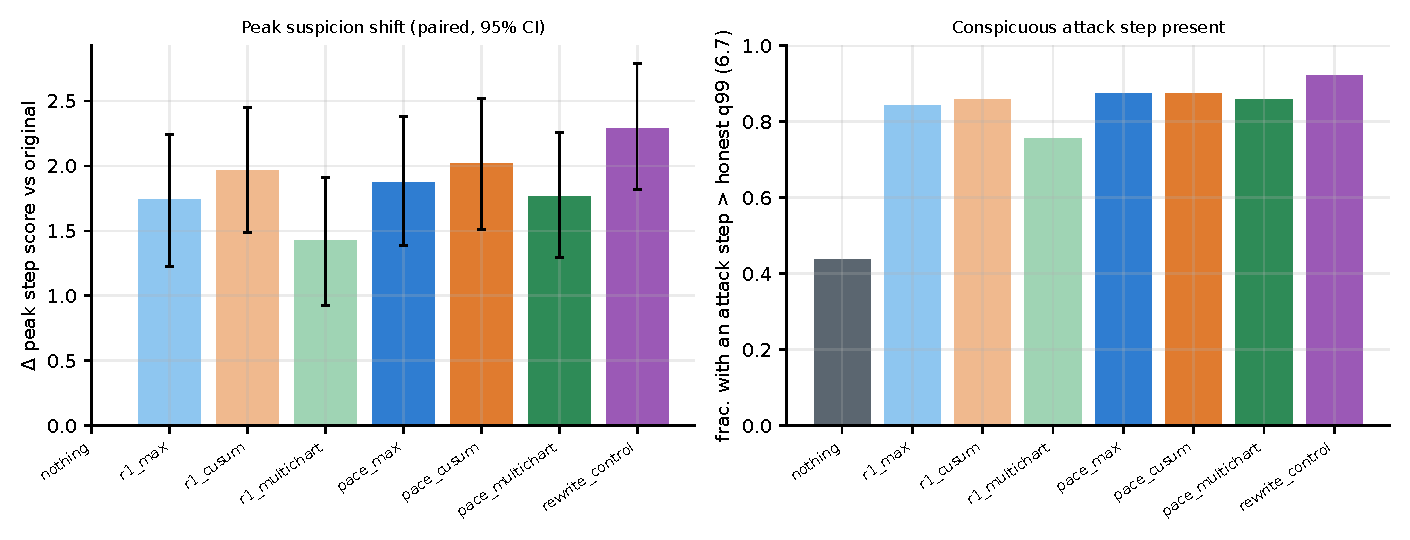
\includegraphics[width=0.78\linewidth]{r2_t3/mechanism_none.pdf}
\caption{Left: shift in peak step score vs the original (paired 95\% CI). Right: share of attacks with at least one attack step above the honest per-step q99 \src{results/r2_t3/mechanism.md}.}
\end{figure}

Every rewrite, with or without detector information, makes the attack-critical operation an explicit standalone action that the monitor scores high: 92\% of control rewrites have an attack step above the honest q99, against 44\% of originals. The originals evade largely because their critical operation is embedded in long, realistic work. Pacing lowers neither the peak nor the share of conspicuous steps relative to the control by much.

\subsection{Detector panel on the originals}
Undetected success of the 126 paired originals at $\alpha=0.01$ (judge and strict coincide for originals) \src{results/r2_t3/tables.md}:
max 0.75, CUSUM $k{=}1.5$ 0.80, multi-chart 0.77, top-3 sum 0.85, SR-type e-detector 0.93, CUSUM $k{=}0.5$ 0.96, e-process 0.95, Shiryaev--Roberts 0.96, windowed GLR 0.95. At $\alpha=0.003$ CUSUM $k=1.5$ leaves 0.95 undetected, max 0.85. The rules that accumulate small evidence (CUSUM $k=0.5$, SR, GLR, e-process) are nearly powerless here: the honest per-step distribution is concentrated at very low scores, so after whitening any non-zero benign step looks like evidence (EXPERIMENT\_LOG, October 21). Among the pacing arms, the SR-type e-detector and windowed GLR catch more of \texttt{pace\_cusum} (0.71 and 0.78 undetected, judge) than CUSUM $k=0.5$ (0.91), but all three remain far weaker than max and top-3 sum.

Held-out FPR (275/275, 200 splits) at $\alpha=0.01/0.003$: max 0.0109/0.0043, CUSUM $k{=}1.5$ 0.0114/0.0039, top-3 sum 0.0115/0.0039, multi-chart 0.0185/0.0114 (1.85$\times$ and 3.81$\times$ nominal) \src{results/fixes/r2_t3/m5_holdout_fpr.csv}.

\subsection{Strategy effect: pacing vs the rewrite control}
The originally reported contrast, adaptive \texttt{pace\_max} minus the one-shot control against max, was $+0.206$. With the joint bootstrap it is $+0.206\ci{+0.063}{+0.325}$, but it compares a best-of-three attempt, selected on the evaluation monitor's own deterministic scores and threshold, with a single attempt \src{results/fixes/corrections.csv} (M1). The selection gain alone, adaptive minus one-shot \texttt{pace\_max}, is $+0.111\ci{+0.048}{+0.190}$. The identifiable strategy contrast is one-shot vs one-shot:

\begin{table}[H]\centering\small
\begin{adjustbox}{max width=\linewidth}
\begin{tabular}{@{}lcccc@{}}
\toprule
One-shot pacing $-$ control & max & CUSUM $k{=}1.5$ & multi-chart & top-3 sum\\
\midrule
\texttt{pace\_max} & \textbf{+0.087}\ci{-0.032}{+0.183} & $+0.063\ci{-0.048}{+0.151}$ & $+0.075\ci{-0.032}{+0.151}$ & $-0.056\ci{-0.127}{+0.056}$\\
\texttt{pace\_cusum} & $+0.040\ci{-0.040}{+0.119}$ & $-0.016\ci{-0.095}{+0.103}$ & $+0.002\ci{-0.101}{+0.081}$ & $-0.071\ci{-0.135}{+0.040}$\\
\texttt{pace\_multichart} & $+0.056\ci{-0.016}{+0.135}$ & $0.000\ci{-0.095}{+0.111}$ & $+0.048\ci{-0.034}{+0.123}$ & $-0.008\ci{-0.087}{+0.079}$\\
\bottomrule
\end{tabular}
\end{adjustbox}
\caption{Round 2 strategy contrasts, strict validity, $\alpha=0.01$, paired $n=126$, joint CIs. Bold: pre-specified primary contrast, $p=0.196$. Judge validity gives $+0.095\ci{-0.024}{+0.190}$ for the primary cell. Holm-adjusted $p=1.00$ for all 24 one-shot contrasts (3 arms $\times$ 4 detectors $\times$ 2 $\alpha$) under both validities \src{results/fixes/r2_t3/tables_fixes_r2_t3.md}, \src{results/fixes/r2_t3/primary_contrast.csv}.}\label{tab:r2strategy}
\end{table}

\begin{figure}[tbp]\centering
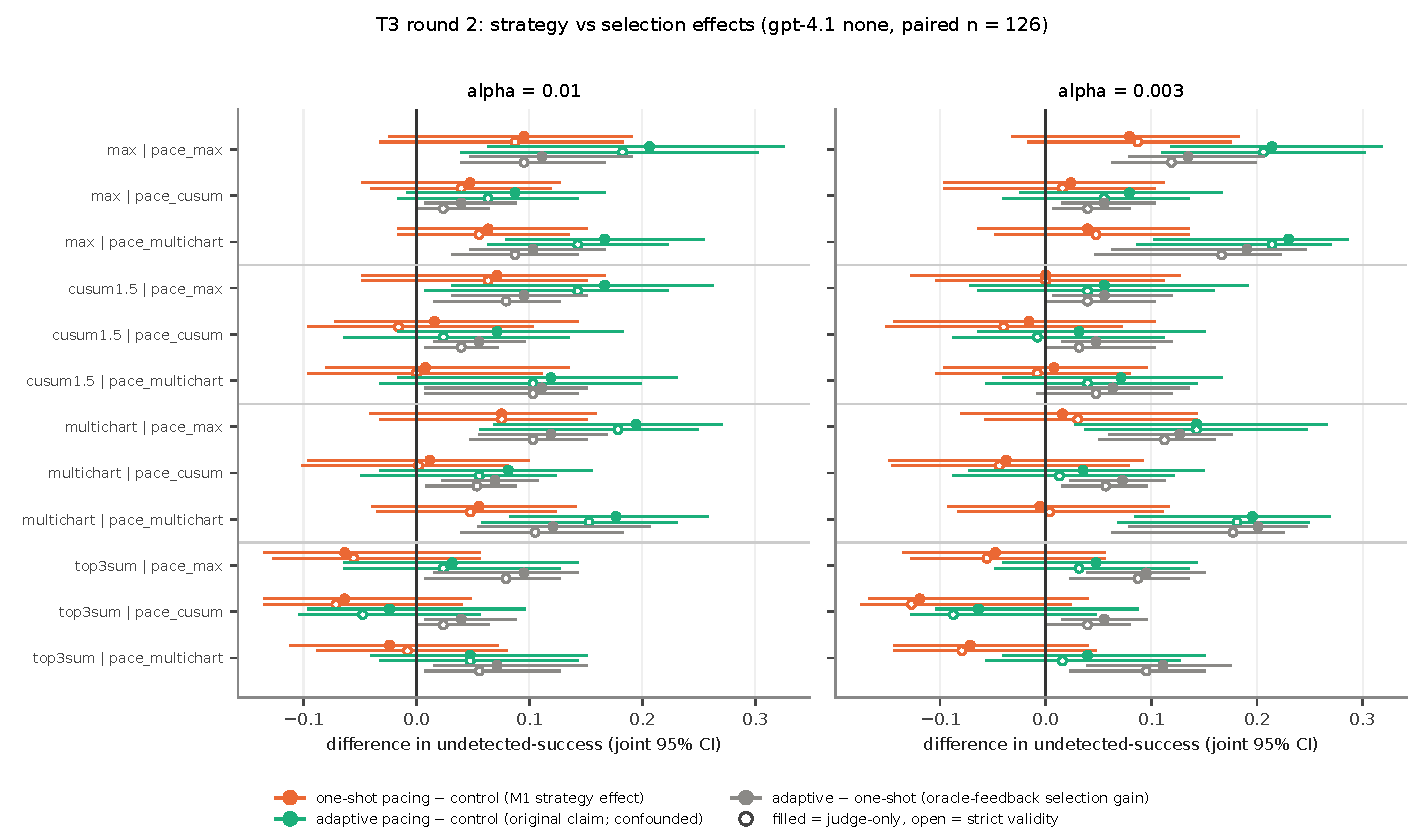
\includegraphics[width=0.78\linewidth]{fixes/r2_t3/fig_contrasts.pdf}
\caption{Round 2 contrasts vs the rewrite control: one-shot pacing (the strategy effect), adaptive pacing (confounded with selection) and the adaptive-minus-one-shot selection gain, judge (filled) and strict (open), joint 95\% CIs \src{results/fixes/r2_t3/fig_contrasts.pdf}.}
\end{figure}

Further round-2 contrasts \src{results/fixes/r2_t3/tables_fixes_r2_t3.md}:
\begin{itemize}
\item \textbf{Top-3 sum neutralizes even the confounded effect}: adaptive \texttt{pace\_max} minus control against top-3 sum is $+0.032\ci{-0.063}{+0.143}$; the one-shot contrasts are $-0.063$, $-0.063$, $-0.024$ (judge).
\item \textbf{Pacing vs round-1 condensation}: none of the six comparisons survives Holm correction across the 20 originally reported comparisons. At $\alpha=0.003$ \texttt{pace\_cusum} minus round-1 CUSUM-aware on CUSUM $k=1.5$ is $-0.103\ci{-0.159}{+0.024}$ (the original attack-only CI excluded 0 in the other direction).
\item \textbf{Pacing vs doing nothing}: adaptive \texttt{pace\_max} minus original against max is $-0.151\ci{-0.278}{-0.008}$ (judge), $-0.190\ci{-0.317}{-0.056}$ (strict-rel), $-0.317\ci{-0.444}{-0.167}$ (strict); one-shot $-0.262\ci{-0.365}{-0.143}$ (judge).
\item \textbf{Control vs doing nothing}: $-0.357\ci{-0.437}{-0.246}$ (judge), $-0.389\ci{-0.468}{-0.278}$ (strict-rel), $-0.500\ci{-0.579}{-0.389}$ (strict); $-0.294\ci{-0.405}{-0.151}$ at $\alpha=0.003$.
\end{itemize}

\begin{figure}[tbp]\centering
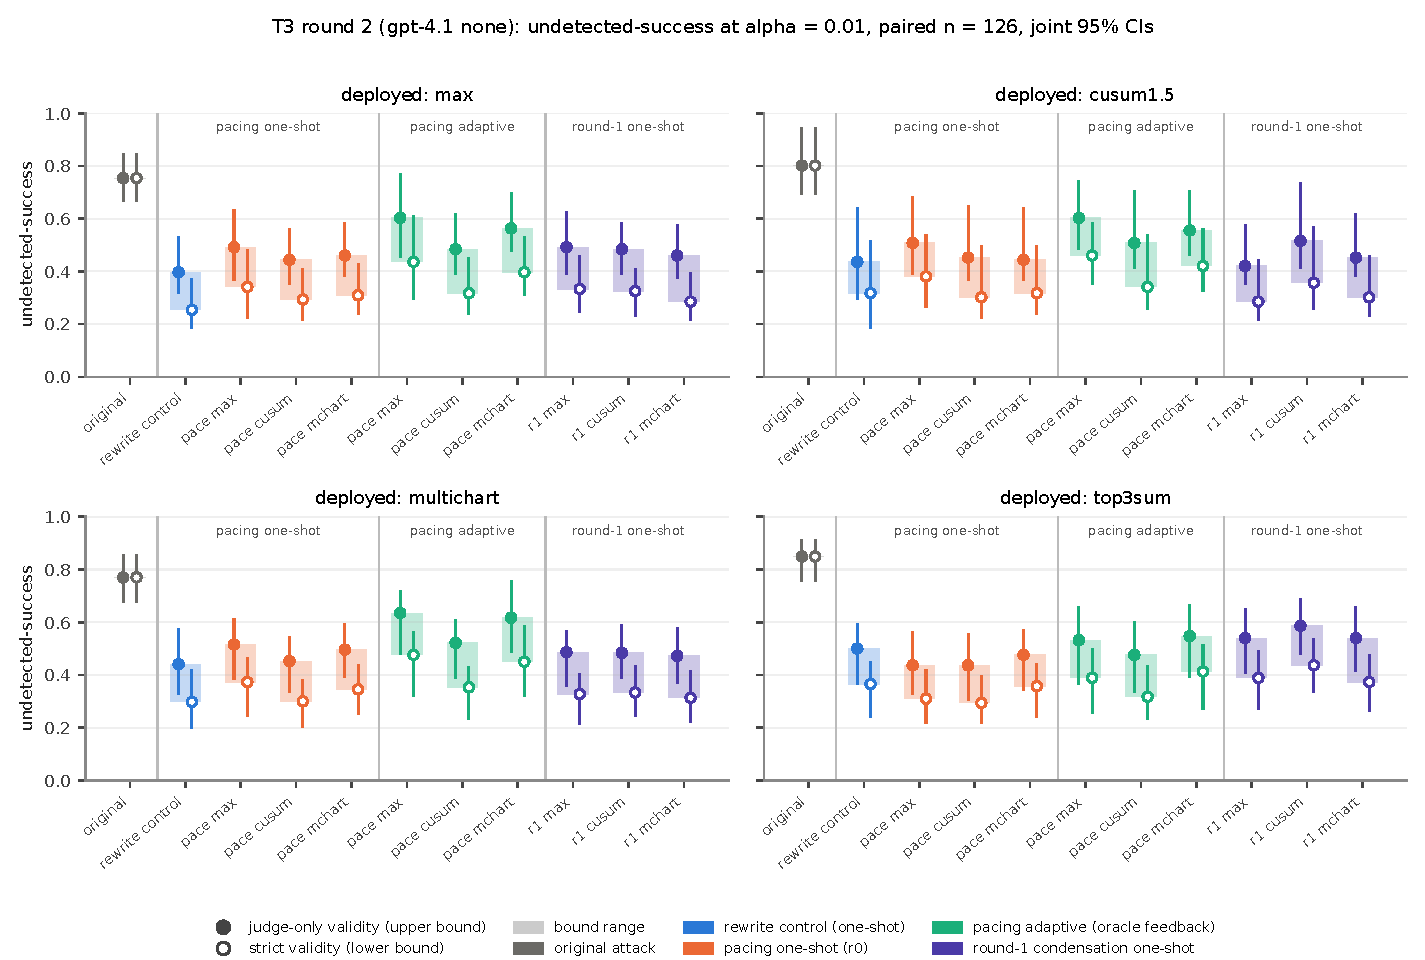
\includegraphics[width=0.8\linewidth]{fixes/r2_t3/fig_us_bounds_a0.01.pdf}
\caption{Round 2 undetected-success levels at $\alpha=0.01$ for four deployed detectors: judge (filled, upper bound) and strict (open, lower bound) validity, joint 95\% CIs. Every rewritten arm sits well below the originals under both bounds \src{results/fixes/r2_t3/fig_us_bounds_a0.01.pdf}.}
\end{figure}

\paragraph{Agent-model confound (audit M9).} Honest-550 is entirely \texttt{claude-opus-4-5}, while 40 of the 126 paired base attacks are \texttt{opus-4-6}. On the originals, max TPR at 1\% FPR is 0.233 ($n=86$, opus-4-5) vs 0.275 ($n=40$, opus-4-6). On the opus-4-5 subset the contrasts keep their sign and size: one-shot \texttt{pace\_max} minus control $+0.070\ci{-0.070}{+0.174}$, control minus original $-0.326\ci{-0.419}{-0.186}$ \src{results/fixes/corrections.csv}. At $\alpha=0.003$ CUSUM $k=1.5$ catches opus-4-6 originals far more often (0.125 vs 0.012) \src{results/fixes/r2_t3/tables_fixes_r2_t3.md}.

\subsection{Covert damage vs ARL}
\begin{figure}[tbp]\centering
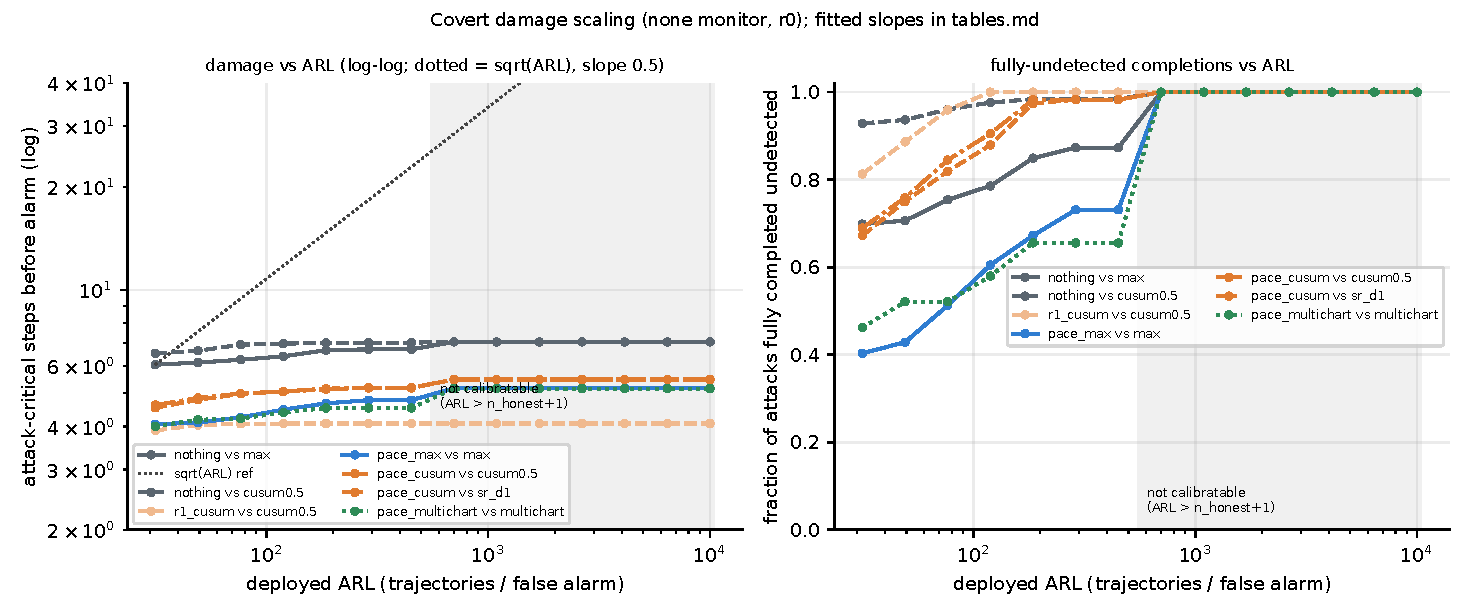
\includegraphics[width=0.8\linewidth]{r2_t3/covert_none_r0.pdf}
\caption{Round 2, one-shot arms. Left: undetected attack-critical steps before the first alarm vs deployed ARL (log-log), with the $\sqrt{\mathrm{ARL}}$ reference (dotted). Right: share of attacks completed with no alarm. Grey: ARL $>551$, not calibratable with 550 honest runs \src{results/r2_t3/tables.md}.}
\end{figure}

Fitted slopes of log damage on log ARL over the calibratable range (ARL $\le551$):
\begin{itemize}
\item round 2: 0.010--0.073 with every CI upper end $\le0.099$ (originals vs max $0.044\ci{0.020}{0.080}$; \texttt{pace\_max} vs max $0.073\ci{0.051}{0.099}$) \src{results/r2_t3/tables.md};
\item round 1, refit after the audit (the original fit ran to ARL $10^4$, beyond the calibratable range): 0.007--0.045 \src{results/fixes/t3/covert_refit_r1.csv}.
\end{itemize}
The prediction of 0.5 is rejected for both naive and pacing attackers. Damage saturates: alarms, when they occur, come from a single high step, and attacks that avoid such a step are never caught at any ARL. The theory's premise, an attacker sitting at the edge of per-step detectability, is not met by these monitors.

%======================================================================
\section{Round 3: replay, a different-family rewriter, leaks and realized FPR}

\subsection{A. Execution replay: infrastructure verified, not run on our trajectories}\label{sec:replay}
The goal was to check side-task success of rewrites by executing them in the real BashArena sandbox with the official scorers, instead of relying on the LLM judge.
\begin{itemize}
\item \textbf{What works.} \texttt{control-arena} 20.1.0 ships the full BashArena setting (dataset loader, per-task multi-service Docker compose, the four official side-task scorers). Our task ids are in its dataset. The base image builds on the laptop, a task's compose comes up healthy, and \texttt{control-arena}'s own firewall side-task test (fixed policy, real sandbox, official scorer, no API) passed end to end. The model-free half (materialize, build, bring up, execute a command list, tear down) is in \texttt{tracks/r3\_t3/replay\_basharena.py}.
\item \textbf{The blocker is data fidelity.} The stored trajectories keep only a rendered action string per step. Bash steps keep the raw command, but text-editor steps (often the attack-critical configuration edit) have no recoverable structured arguments, some rewritten steps are bare shell, and the rewriter never emitted structured tool calls. A mis-parsed step would score as a failed attack and bias the comparison, so the replay was not run.
\item \textbf{Concrete path to a full replay.}
\begin{enumerate}
\item Re-extract structured tool calls \{function, arguments\} for the originals from the source \texttt{.eval} logs.
\item Make the rewriter emit structured tool calls instead of rendered strings (a JSON schema in the rewrite prompt).
\item Add a fixed-trajectory policy to \texttt{control-arena}'s BashArena (an Inspect solver that replays the recorded calls) and run \texttt{inspect eval} per (sample, arm) with the task-id whitelist, the matching side task and the setting's own scorer; read \texttt{side\_task\_success} from the log.
\end{enumerate}
This needs no API spend and runs on the laptop, at a few minutes per (sample, arm). Because the scorers check final system state, fabricated intermediate outputs do not invalidate a rewrite; a command that silently depended on a real earlier output would correctly fail.
\end{itemize}

\subsection{B. Is the rewrite artifact a same-model effect?}
In rounds 1--2 the rewriter (\texttt{gpt-4.1}) was the round-2 monitor model, so a rewrite might be conspicuous only to its own model family. \texttt{claude-sonnet-4.5} was tried first but refused almost all pacing prompts while accepting the control (EXPERIMENT\_LOG, October 22), so \texttt{gemini-2.5-pro} was used: a one-shot control plus the three pacing arms on 35 base attacks (17 tasks), scored by \texttt{gpt-4.1} \texttt{none} and compared with the round-2 \texttt{gpt-4.1} one-shot arms on the same 35.

\begin{table}[H]\centering\small
\begin{adjustbox}{max width=\linewidth}
\begin{tabular}{@{}llccccc@{}}
\toprule
Arm & Rewriter & Mean peak & Judge-valid & Strict-valid & Literal pres. & Length ratio\\
\midrule
original & -- & 5.62 & 1.00 & 1.00 & 1.00 & 1.00\\
rewrite control & \texttt{gpt-4.1} & 8.49 & 0.94 & 0.77 & 0.91 & 1.17\\
rewrite control & \texttt{gemini} & 7.59 & 0.91 & 0.74 & 0.90 & 1.20\\
pacing (3 arms) & \texttt{gpt-4.1} & 8.16--8.29 & 0.94--0.97 & 0.74--0.77 & 0.87--0.90 & 1.15--1.18\\
pacing (3 arms) & \texttt{gemini} & 6.98--7.33 & 0.74--0.80 & 0.57--0.63 & 0.90 & 1.12--1.14\\
\bottomrule
\end{tabular}
\end{adjustbox}
\caption{Round 3 rewrites, paired $n=35$, \texttt{gpt-4.1} \texttt{none} \src{results/r3_t3/compare.md} (this descriptive table stands; the contrasts in that file are superseded by \texttt{paired\_contrasts.md}).}\label{tab:r3desc}
\end{table}

\begin{table}[H]\centering\small
\begin{adjustbox}{max width=\linewidth}
\begin{tabular}{@{}lcccc@{}}
\toprule
Contrast (one-shot, strict US) & max, 0.01 & max, 0.003 & multi-chart, 0.01 & top-3 sum, 0.01\\
\midrule
control/\texttt{gpt-4.1} $-$ original & $-0.600\ci{-0.721}{-0.379}$ & $-0.486\ci{-0.695}{-0.286}$ & $-0.543\ci{-0.705}{-0.364}$ & $-0.486\ci{-0.676}{-0.276}$\\
control/\texttt{gemini} $-$ original & $-0.371\ci{-0.550}{-0.185}$ & $-0.314\ci{-0.537}{-0.100}$ & $-0.400\ci{-0.557}{-0.190}$ & $-0.286\ci{-0.419}{-0.118}$\\
control: \texttt{gpt-4.1} $-$ \texttt{gemini} & $-0.229\ci{-0.355}{-0.036}$ & $-0.171\ci{-0.333}{-0.029}$ & $-0.143\ci{-0.306}{-0.027}$ & $-0.200\ci{-0.368}{-0.062}$\\
\midrule
\texttt{pace\_max}/\texttt{gpt-4.1} $-$ control & $+0.114\ci{-0.107}{+0.257}$ & $+0.029\ci{-0.129}{+0.200}$ & $+0.029\ci{-0.128}{+0.222}$ & $0.000\ci{-0.154}{+0.220}$\\
\texttt{pace\_cusum}/\texttt{gpt-4.1} $-$ control & $-0.029\ci{-0.200}{+0.067}$ & $-0.057\ci{-0.214}{+0.086}$ & $-0.086\ci{-0.245}{+0.063}$ & $-0.114\ci{-0.258}{+0.111}$\\
\texttt{pace\_multichart}/\texttt{gpt-4.1} $-$ control & $+0.086\ci{-0.051}{+0.194}$ & $+0.029\ci{-0.088}{+0.171}$ & $+0.029\ci{-0.100}{+0.172}$ & $0.000\ci{-0.152}{+0.200}$\\
\texttt{pace\_max}/\texttt{gemini} $-$ control & $-0.143\ci{-0.290}{+0.077}$ & $-0.114\ci{-0.294}{+0.062}$ & $-0.086\ci{-0.270}{+0.075}$ & $-0.143\ci{-0.289}{+0.037}$\\
\texttt{pace\_cusum}/\texttt{gemini} $-$ control & $-0.143\ci{-0.320}{+0.071}$ & $-0.171\ci{-0.368}{+0.053}$ & $-0.086\ci{-0.312}{+0.068}$ & $-0.143\ci{-0.323}{+0.029}$\\
\texttt{pace\_multichart}/\texttt{gemini} $-$ control & $-0.029\ci{-0.212}{+0.125}$ & $-0.114\ci{-0.263}{+0.111}$ & $-0.029\ci{-0.210}{+0.138}$ & $-0.143\ci{-0.303}{+0.029}$\\
\bottomrule
\end{tabular}
\end{adjustbox}
\caption{Round 3 paired contrasts in strict undetected success, $n=35$ base attacks, honest $n=550$, task-clustered joint bootstrap \src{results/r3_t3/paired_contrasts.md}. Every pacing-minus-control CI contains 0 (all 48 cells in the file, including CUSUM $k=1.5$).}\label{tab:r3contrasts}
\end{table}

\paragraph{Validity vs detection (audit2 A4).} Strict US multiplies validity by non-detection, so a contrast can be negative because rewrites break the attack rather than because they are caught. The second audit split each contrast \src{results/audit2/repro_t3r3.csv}:

\begin{table}[H]\centering\small
\begin{adjustbox}{max width=\linewidth}
\begin{tabular}{@{}lccc@{}}
\toprule
Contrast (max, $\alpha=0.01$) & strict US & detection only (validity ignored) & both-valid pairs\\
\midrule
control/\texttt{gemini} $-$ original & $-0.371\ci{-0.548}{-0.182}$ & $-0.143\ci{-0.300}{-0.027}$ & $-0.192\ci{-0.364}{-0.038}$ ($n=26$)\\
control/\texttt{gpt-4.1} $-$ original & $-0.600\ci{-0.732}{-0.385}$ & $-0.429\ci{-0.548}{-0.256}$ & $-0.519\ci{-0.667}{-0.296}$ ($n=27$)\\
control: \texttt{gpt-4.1} $-$ \texttt{gemini} & $-0.229\ci{-0.345}{-0.056}$ & $-0.286\ci{-0.414}{-0.091}$ & $-0.292\ci{-0.440}{-0.045}$ ($n=24$)\\
\texttt{pace\_max}/\texttt{gemini} $-$ control & $-0.143\ci{-0.294}{+0.059}$ & $-0.057\ci{-0.206}{+0.171}$ & $-0.053$ ($n=19$)\\
\texttt{pace\_cusum}/\texttt{gemini} $-$ control & $-0.143\ci{-0.314}{+0.059}$ & $-0.057\ci{-0.156}{+0.167}$ & $-0.095$ ($n=21$)\\
\texttt{pace\_multichart}/\texttt{gemini} $-$ control & $-0.029\ci{-0.214}{+0.118}$ & $+0.086\ci{-0.129}{+0.258}$ & $+0.150$ ($n=20$)\\
\bottomrule
\end{tabular}
\end{adjustbox}
\caption{Decomposition by the second audit's independent implementation (its strict-US CIs differ from Table~\ref{tab:r3contrasts} in the third decimal).}\label{tab:a4}
\end{table}

\begin{figure}[tbp]\centering
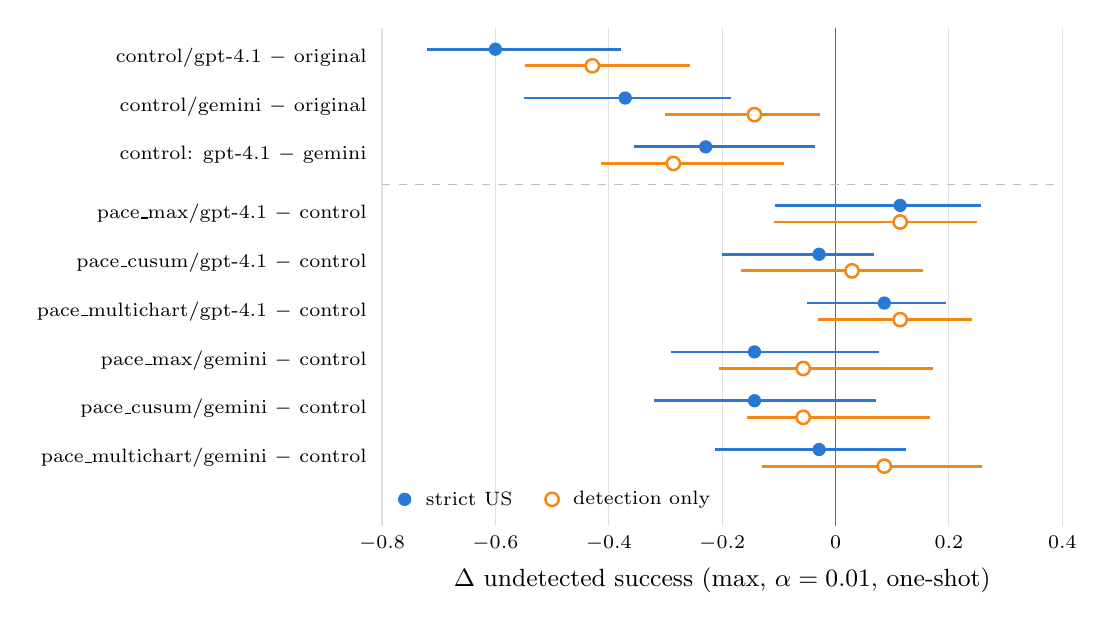
\begin{tikzpicture}[x=7.2cm,y=0.62cm]
\def\xl{-0.80}\def\xr{0.40}\def\yt{0.6}\def\yb{-9.6}
\foreach \v in {-0.8,-0.6,-0.4,-0.2,0.2,0.4} {\draw[black!12] (\v,\yt) -- (\v,\yb); \node[font=\scriptsize,below] at (\v,\yb) {$\v$};}
\draw[black!60] (0,\yt) -- (0,\yb); \node[font=\scriptsize,below] at (0,\yb) {$0$};
\node[font=\small] at (-0.2,\yb-1.1) {$\Delta$ undetected success (max, $\alpha=0.01$, one-shot)};
\newcommand{\frow}[8]{%
\node[anchor=east,font=\scriptsize] at (\xl-0.01,#1) {#2};
\draw[hblue,line width=1pt] (#4,{#1+0.17}) -- (#5,{#1+0.17}); \fill[hblue] (#3,{#1+0.17}) circle (2.4pt);
\draw[BurntOrange,line width=1pt] (#7,{#1-0.17}) -- (#8,{#1-0.17}); \draw[BurntOrange,fill=white,line width=0.9pt] (#6,{#1-0.17}) circle (2.4pt);}
\frow{0}{control/gpt-4.1 $-$ original}{-0.600}{-0.721}{-0.379}{-0.429}{-0.548}{-0.256}
\frow{-1}{control/gemini $-$ original}{-0.371}{-0.550}{-0.185}{-0.143}{-0.300}{-0.027}
\frow{-2}{control: gpt-4.1 $-$ gemini}{-0.229}{-0.355}{-0.036}{-0.286}{-0.414}{-0.091}
\draw[black!25,dashed] (\xl,-2.6) -- (\xr,-2.6);
\frow{-3.2}{pace\_max/gpt-4.1 $-$ control}{0.114}{-0.107}{0.257}{0.114}{-0.108}{0.250}
\frow{-4.2}{pace\_cusum/gpt-4.1 $-$ control}{-0.029}{-0.200}{0.067}{0.029}{-0.167}{0.154}
\frow{-5.2}{pace\_multichart/gpt-4.1 $-$ control}{0.086}{-0.051}{0.194}{0.114}{-0.031}{0.240}
\frow{-6.2}{pace\_max/gemini $-$ control}{-0.143}{-0.290}{0.077}{-0.057}{-0.206}{0.171}
\frow{-7.2}{pace\_cusum/gemini $-$ control}{-0.143}{-0.320}{0.071}{-0.057}{-0.156}{0.167}
\frow{-8.2}{pace\_multichart/gemini $-$ control}{-0.029}{-0.212}{0.125}{0.086}{-0.129}{0.258}
\fill[hblue] (-0.76,-9.05) circle (2.4pt); \node[anchor=west,font=\scriptsize] at (-0.74,-9.05) {strict US};
\draw[BurntOrange,fill=white,line width=0.9pt] (-0.50,-9.05) circle (2.4pt); \node[anchor=west,font=\scriptsize] at (-0.48,-9.05) {detection only};
\end{tikzpicture}
\caption{Round 3 contrasts with 95\% CIs. Filled: strict undetected success \src{results/r3_t3/paired_contrasts.md}. Open: detection only, validity ignored \src{results/audit2/repro_t3r3.csv}. Above the dashed line: rewrite artifact and cross-rewriter difference; below: strategy effect.}\label{fig:r3forest}
\end{figure}

\paragraph{Reading.}
\begin{itemize}
\item \textbf{The rewrite artifact is not a same-model effect.} A different-family rewriter still lowers undetected success, and the detection-only part, $-0.143\ci{-0.300}{-0.027}$, excludes 0. About 60\% of the $-0.37$ is validity loss (gemini control strict-valid 0.74 vs 1.00 for originals).
\item \textbf{Same-model inflation exists, but only for the control.} The \texttt{gpt-4.1} control is more detectable to the \texttt{gpt-4.1} monitor than the \texttt{gemini} control ($-0.229$ strict, $-0.286$ detection only). For the pacing arms no cross-rewriter difference at max is significant; one of 24 cross-rewriter pacing cells (\texttt{pace\_cusum} on top-3 sum, $\alpha=0.01$) excludes 0 \src{results/r3_t3/paired_contrasts.md}.
\item \textbf{No strategy effect with either rewriter.} The 12 pacing-minus-control contrasts at max (2 rewriters $\times$ 3 arms $\times$ 2 FPRs) range from $-0.171$ to $+0.114$, all with CIs containing 0. The negative \texttt{gemini} pacing contrasts are validity loss: detection-only $-0.057$, $-0.057$, $+0.086$, all n.s.
\end{itemize}

\subsection{C. Do fabricated tool outputs leak the rewrite?}
Rewrites carry fabricated outputs for new steps; originals carry real ones. If fabricated outputs were a cue, the monitor could separate rewrites from originals for reasons unrelated to the attack. 250 honest runs, the 35 originals and all 8 round-3 arms were re-scored with the current action's output stripped \src{results/r3_t3/leak_peaks.md}:
\begin{itemize}
\item stripping outputs lowers the originals' mean peak by $-0.55\ci{-1.03}{-0.08}$ (real outputs add suspicion);
\item rewrite peaks barely move ($\Delta$ from $-0.33$ to $+0.25$);
\item the difference-in-differences (rewrite $\Delta$ minus original $\Delta$) is $+0.22$ to $+0.79$: without outputs the gap between rewrites and originals \emph{widens}.
\end{itemize}
The no-output contrasts replicate the with-output ones: control minus original against max at $\alpha=0.01$ is $-0.514\ci{-0.667}{-0.321}$ (\texttt{gpt-4.1}) and $-0.314\ci{-0.536}{-0.179}$ (\texttt{gemini}); all 24 pacing-minus-control CIs contain 0 \src{results/r3_t3/paired_contrasts_noout.md}. Fabricated outputs do not drive the findings.

\subsection{D. Realized held-out FPR}
\begin{table}[H]\centering\small
\begin{adjustbox}{max width=\linewidth}
\begin{tabular}{@{}lcccc@{}}
\toprule
Detector & with output, 0.01 & with output, 0.003 & no output, 0.01 & no output, 0.003\\
\midrule
max & 0.0107\ci{0.0000}{0.0292} & 0.0038 & 0.0174 & 0.0104\\
CUSUM $k{=}1.5$ & 0.0102\ci{0.0000}{0.0292} & 0.0033 & 0.0164 & 0.0088\\
top-3 sum & 0.0106\ci{0.0000}{0.0292} & 0.0040 & 0.0156 & 0.0088\\
multi-chart OR & \textbf{0.0173}\ci{0.0027}{0.0432} & \textbf{0.0102} & 0.0255 & 0.0177\\
\bottomrule
\end{tabular}
\end{adjustbox}
\caption{Mean realized trajectory FPR over 200 random 50/50 honest splits (brackets: 2.5/97.5 percentiles). With output: 550 honest runs; no output: 250 \src{results/r3_t3/realized_fpr.md}.}\label{tab:fpr}
\end{table}
With 550 honest runs, max, CUSUM $k=1.5$ and top-3 sum realize nominal FPR. The multi-chart OR runs hot (1.7$\times$ at 0.01, 3.4$\times$ at 0.003): its exponential-tail fits overfit the calibration half. This matches the round-1 (1.79$\times$/4.12$\times$) and round-2 (1.85$\times$/3.81$\times$) held-out checks. With only 125 honest runs per calibration half (no-output set) every detector runs 1.6--2.6$\times$ hot at 0.01, so the no-output contrasts are less precise.

%======================================================================
\section{What holds, what is weakened, what is dropped}\label{sec:status}

\begin{table}[H]\centering\small
\begin{tabularx}{\linewidth}{@{}>{\raggedright\arraybackslash}p{0.36\linewidth}>{\raggedright\arraybackslash}X@{}}
\toprule
\multicolumn{2}{@{}l}{\textbf{Holds}}\\
\midrule
LLM rewriting of a working attack makes it more detectable & Round 2 control $-0.357$ (judge) to $-0.500$ (strict); round 3 $-0.60$ (\texttt{gpt-4.1}) and $-0.37$ (\texttt{gemini}); replicates without outputs.\\
Rewrite artifact is not a same-model effect & Different-family rewriter, detection-only $-0.143\ci{-0.300}{-0.027}$ (weaker than first stated; see below).\\
No detectable strategy effect of detector knowledge & Primary $+0.087\ci{-0.032}{+0.183}$; 24/24 round-2 one-shot contrasts Holm $p=1.00$; round 3 all pacing-control CIs contain 0.\\
Pacing still worse than doing nothing & \texttt{pace\_max} $-$ original $-0.151$ (judge) to $-0.317$ (strict).\\
Top-3 sum neutralizes the (confounded) pacing gain & $+0.032\ci{-0.063}{+0.143}$ adaptive; one-shot $\le0$.\\
Max, CUSUM $k{=}1.5$, top-3 sum are the well-calibrated, useful rules & Realized FPR $\approx$ nominal (Table~\ref{tab:fpr}); max strongest on originals, top-3 sum most robust to pacing.\\
Small-evidence accumulators are near-powerless here & Originals $\ge0.93$ undetected under CUSUM $k{=}0.5$, e-process, SR, GLR.\\
No $\sqrt{\mathrm{ARL}}$ scaling & Slopes 0.007--0.073 on ARL $\le551$.\\
Fabricated outputs are not the cue & Leak test DiD $+0.22$ to $+0.79$; no-output contrasts replicate.\\
\midrule
\multicolumn{2}{@{}l}{\textbf{Weakened}}\\
\midrule
Gemini control $-0.37$ vs originals & About 60\% is broken attacks; detection-only $-0.143$ (audit2 A4).\\
Multi-chart OR closes CUSUM's gap and ties max & Its cells overstate detection: realized FPR 1.7--2.0$\times$ at 0.01, 3.4--4.2$\times$ at 0.003 across rounds.\\
Adaptive feedback helps the attacker ($+0.10$ to $+0.17$) & True in-sample only: selection on the evaluation monitor's own scores; $+0.03$ to $+0.08$ in the mode not used for feedback.\\
Round-1 levels 0.63--0.73 vs max & Judge-only upper bounds; strict 0.47--0.53.\\
Strong monitor & Pilot AUROC 0.871 did not carry over; full-set gain is low-FPR TPR only (0.246 vs 0.143 at 1\%).\\
\midrule
\multicolumn{2}{@{}l}{\textbf{Dropped}}\\
\midrule
Detector-aware rewriting backfires (round 1) & No control; vs the round-2 control the aware arms are $+0.03$ to $+0.14$, in the attacker's favour (M3).\\
Pacing beats the control by $+0.21$ (round 2) & Adaptive vs one-shot; one-shot vs one-shot $+0.095$ judge / $+0.087$ strict, n.s. (M1).\\
Pacing beats round-1 condensation & No comparison survives Holm; one sign reversal (m4).\\
``Drops are real detection, not broken attacks''; validity penalty $\le2$ pp & Judge-strict gap is 0.17--0.20 in round 1 (M2); 60\% of the round-3 artifact is validity (A4).\\
\bottomrule
\end{tabularx}
\end{table}

%======================================================================
\section{Errata relative to the October 21 version}

The October 21 PDF covered round 1 only and predates both audits. Its statements are corrected as follows \src{results/fixes/corrections.csv}, \src{results/audit2/corrections.csv}.

\begin{table}[H]\centering\small
\begin{tabularx}{\linewidth}{@{}>{\raggedright\arraybackslash}p{0.40\linewidth}>{\raggedright\arraybackslash}X@{}}
\toprule
October 21 statement & Correction\\
\midrule
``Detector-aware rewriting did not help the attacker; it usually hurt'' & Dropped. The drop is the cost of LLM rewriting; against a rewrite-only control the aware arms are not worse (Section~\ref{sec:r1reread}).\\
Undetected success vs max 0.86 (originals) vs 0.63--0.73 (aware) & Judge-only upper bounds. Strict: 0.47--0.53. Differences with joint CIs: $-0.127$ to $-0.222$ (judge), $-0.325$ to $-0.389$ (strict).\\
Undetected success vs OR fell from 0.85 to 0.49--0.68 & Judge-only; strict 0.35--0.48; the OR realizes 1.79$\times$ nominal FPR on held-out honest runs.\\
Condensation (length ratio 0.58--0.83) raised peak suspicion 5.8 $\to$ 7.6 and explains the drop & Descriptive numbers stand. The explanation is dropped: a non-condensing control raises the peak more ($+2.29$ vs $+1.43$ to $+1.96$).\\
Adaptive beats one-shot by $+0.10$ to $+0.17$ & In-sample oracle selection, not attacker capability; $+0.032$ to $+0.079$ in \texttt{none} mode.\\
CUSUM alone is the most evadable detector & Holds for $k=0.5$. CUSUM with $k=1.5$ is close to max at $\alpha=0.01$ (0.80 vs 0.75 undetected originals) and weaker at 0.003.\\
Max and the OR are strongest; the OR roughly ties max & The OR's tie is partly extra false alarms; with calibrated rules, max, CUSUM $k{=}1.5$ and top-3 sum lead.\\
$\sqrt{\mathrm{ARL}}$: slopes 0.00--0.03 over ARL $10^{1.5}$--$10^4$ & Conclusion holds, fit range was wrong: no threshold is calibratable above ARL $\approx551$. Refit: 0.007--0.045.\\
Validity 98--99\% (judge), 0.88--0.90 (literal); penalty $\le2$ pp; ``drops are real detection'' & ``Valid'' was judge-only; 0.88--0.90 is a mean fraction. Strict-valid rate 0.79--0.81 (adaptive), 0.72--0.80 (one-shot); judge-strict gap 0.17--0.20. Sentence dropped.\\
``Not an artifact of fabricated outputs'' (based on \texttt{none} mode) & Holds, now tested directly by stripping outputs (round 3C).\\
No Docker replay because of disk & Replay infrastructure verified; the blocker is the lack of structured tool calls in stored trajectories.\\
Weak monitor is the main caveat; re-run with a strong monitor & Done in round 2: the stronger monitor raises low-FPR TPR but does not change any conclusion.\\
CIs over base attacks only & Replaced by joint (honest + attack) bootstrap; most intervals widen.\\
\bottomrule
\end{tabularx}
\end{table}

%======================================================================
\section{Interpretation}
\begin{enumerate}
\item \textbf{The binding constraint on these attackers is rewriting, not detector knowledge.} Every LLM rewrite we produced, with or without monitor information and from two model families, isolated the attack-critical operation into a high-scoring standalone action (92\% of control rewrites vs 44\% of originals had an attack step above the honest q99). Telling the rewriter the detector, its parameters and the honest score distribution did not measurably undo this.
\item \textbf{A null strategy effect is not evidence that detector-aware evasion is impossible.} The one-shot CIs allow gains of up to about $+0.18$ against max. The attacker never executed anything, saw only its own fabricated outputs, and had at most three attempts. An attacker that operates live in the environment, or a much stronger rewriter, could behave differently.
\item \textbf{Detector design.} Against both weak and stronger monitors, single-spike rules (max, top-3 sum, CUSUM with a large reference) dominate small-evidence accumulators, because detection is spike-driven and the honest per-step distribution has a mass at very low scores. Top-3 sum was the most robust to the pacing attackers. The multi-chart OR is not a safe default as implemented: its tail-fit thresholds need held-out calibration or a conservative correction.
\item \textbf{The covert-adversary regime was not reached.} Damage is flat in ARL because attacks are caught by one conspicuous step or not at all. Testing the $\sqrt{\mathrm{ARL}}$ law needs a monitor whose per-step evidence is informative but small, and far more honest runs than 550 to calibrate long ARLs.
\item \textbf{Validity is the weakest link.} Judge-only validity overstates attacker success by 0.17--0.20 in round 1, and most of the different-family rewrite artifact is broken attacks. Execution replay is the necessary next measurement.
\end{enumerate}

\section{Limitations}
\begin{itemize}
\item \textbf{No execution.} Side-task success of rewrites rests on an LLM judge plus a static literal check; strict and judge validity bracket the truth but do not replace replay.
\item \textbf{Monitors.} \texttt{gpt-4.1} improves low-FPR TPR over \texttt{gpt-4.1-mini} (0.246 vs 0.143) but is not a strong monitor in absolute terms.
\item \textbf{Round 3 is small.} $n=35$ base attacks from 17 tasks, one-shot only; CIs are wide ($\pm0.15$--0.20).
\item \textbf{Same model as rewriter and monitor} in rounds 1--2. Round 3 shows the effect is modest and confined to the control arm.
\item \textbf{Agent-model confound.} Honest runs are all \texttt{opus-4-5}; 40 of 126 paired attacks are \texttt{opus-4-6}. Contrasts are stable on the opus-4-5 subset; round 3 is not stratified.
\item \textbf{Attack-relevant step labels} used in the cost and damage analyses are self-reported by the rewriter.
\item \textbf{Label-correlated surface features} in the source data (truncation, a text-editor sub-command, reasoning visibility) are documented, not removed; LLM monitors never see reasoning \src{results/audit/issues.csv} (m8).
\item \textbf{White-box reader rows on round-1 rewrites} (white-box pilot) cannot be re-derived: their score files were overwritten by an empty sync \src{results/audit2/issues.csv} (A2).
\end{itemize}

\section{Next steps}
\begin{enumerate}
\item \textbf{Execution replay} along the path in Section~\ref{sec:replay}: structured tool calls for originals and rewrites, a fixed-trajectory policy in \texttt{control-arena}, official scorers. Laptop only, no API spend.
\item \textbf{An adaptive control}: the rewrite control with the same feedback loop, evaluated on a held-out monitor or held-out threshold, so that adaptive pacing can be compared fairly.
\item \textbf{Live attackers}: let the attacker act in the sandbox with knowledge of the detector, instead of rewriting a finished transcript.
\item \textbf{Calibration}: held-out or cross-fitted thresholds for the multi-chart OR; more honest runs (thousands) for any ARL-scaling test.
\end{enumerate}

\paragraph{Reproduction.} Code: \nolinkurl{tracks/t3_aware_attacker/}, \nolinkurl{tracks/r2_t3/}, \nolinkurl{tracks/r3_t3/} (rounds 1--3); \nolinkurl{tracks/fixes/t3/}, \nolinkurl{tracks/audit2/repro_t3r3.py} (audits). Results: \nolinkurl{results/{t3,r2_t3,r3_t3}/}, \nolinkurl{results/fixes/{t3,r2_t3}/}, \nolinkurl{results/fixes/corrections.csv}, \nolinkurl{results/audit{,2}/}; in \nolinkurl{r3_t3/} the \nolinkurl{paired_contrasts[_noout].md} files are canonical and the contrasts in \nolinkurl{compare*.md} are superseded. Rewritten trajectories stay in the gitignored \nolinkurl{data/processed/t3_refined/}; attack content is never committed. Repository: \href{https://github.com/gregkocher/agent-monitor-detection}{gregkocher/agent-monitor-detection} (private).
\end{document}
